\section{Two stage approach for hardware optimizations}
\label{sec:twoStage}
To solve the problem of selecting the mode in which to run the perception algorithm to minimize computation energy without having a significant impact on the control performance, we propose a two stage solution. The first stage is offline and is concerned with thoroughly profiling the perception algorithm's throughput ($T(\sigma,F_c,F_g)$) and power consumption ($P(\sigma,F_c,F_g)$) as functions of the hardware knobs ($\sigma$, $F_c$ and $F_g$). The second stage is using this profiled information at run-time to choose a trade-off between computation power and throughput based on the feedback from the controlled system and then picking the task resource allocation schedule $\sigma$ and CPU-GPU ($F_c,F_g$) frequencies which help us best realize this trade-off. A high-level view of this approach is shown in Fig. \ref{fig:juicyj}More details follow.

\begin{figure*}[htbp]
	\centering
	\includegraphics[scale=0.36]{Figs/bigFig.pdf}
	\caption{High level view of the two stage approach.}
	\label{fig:juicyj}%same freq diff assignment}
\end{figure*}

\subsection{Offline profiling of performance and power consumption of the perception algorithm}
\label{sec:profiling}
\begin{figure}
	\centering
	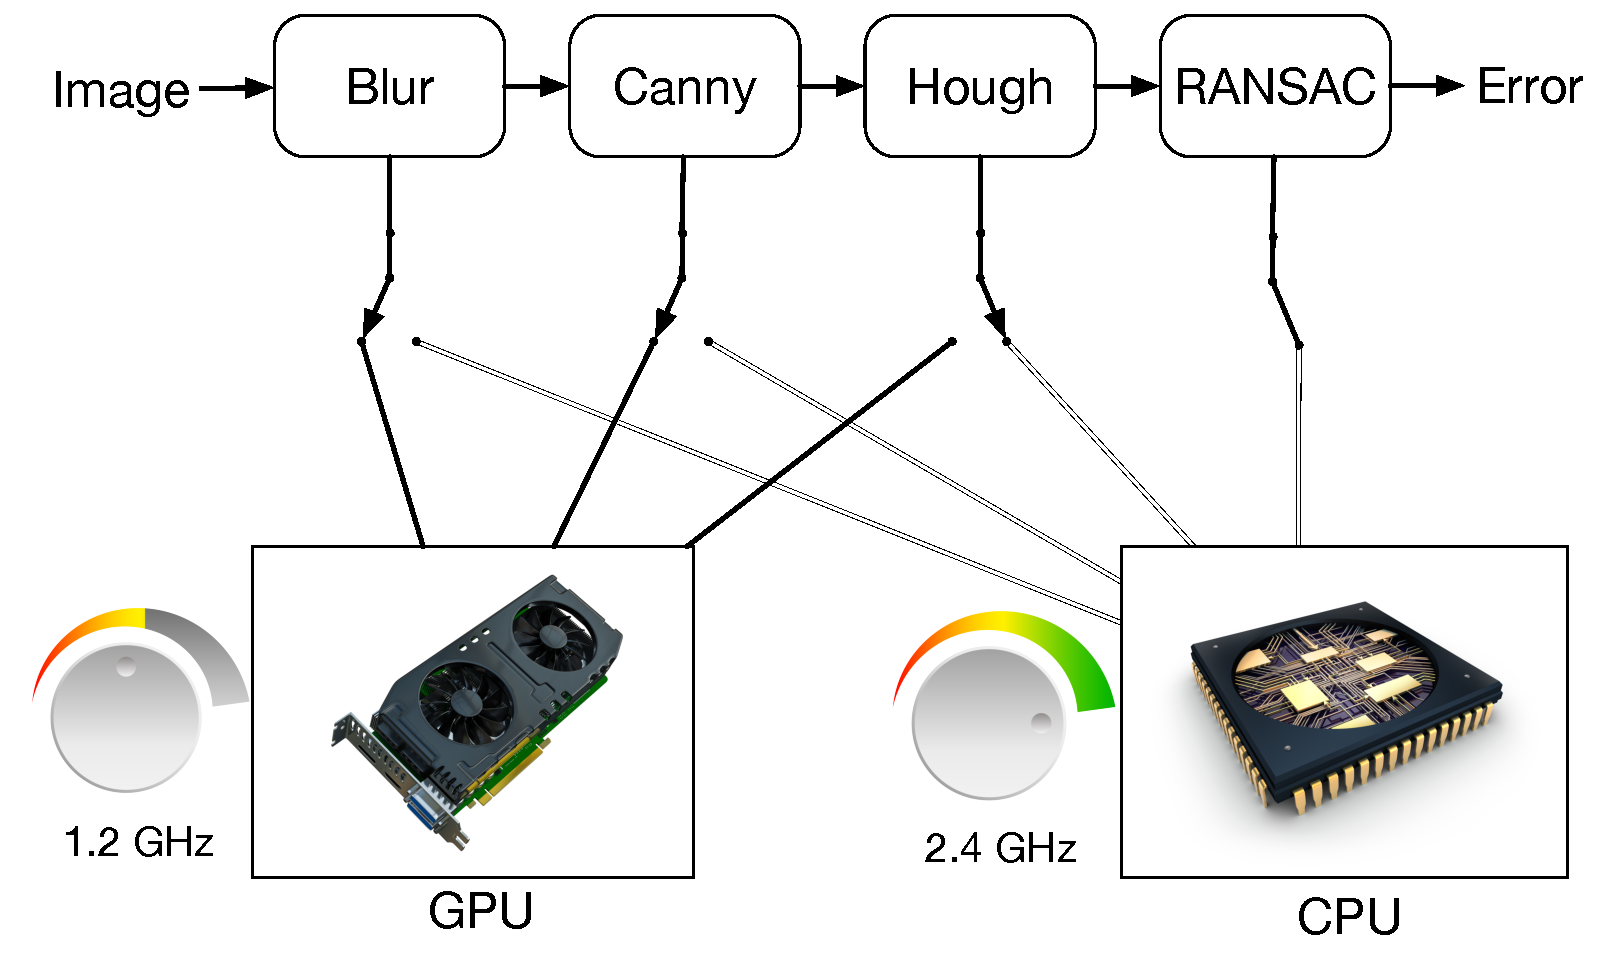
\includegraphics[scale=0.3]{Figs/vanishing}
	\caption{The vanishing point algorithm with components running on either CPU or GPU at various frequencies, resulting in different power consumptions and execution times.}
	\label{fig:vanishing}		
\end{figure}

\subsection{Feedback driven online scheduling and hardware mode selection}
\label{sec:scheduling}
%\subsection{Feedback driven scheduling and hardware mode selection}

From the profiling stage of the perception algorithm \ref{}[section], we know that for a particular scheduling of the components of the algorithm on the CPU or the GPU, we have varying throughput and power consumption profiles with changing CPU-GPU frequencies. With this profile, and the fact that less delay results in better closed loop control performance of a system, we can take a step towards formulating a scheduling (tasks on CPU or GPU) and hardware mode (CPU-GPU frequencies) selection problem to be solved at run-time. Consider maximizing at each time step $t$, a cost function of the form:

\begin{equation}
\max_{\sigma,F_{c},F_{g}} \alpha(t)\mathbf{\bar{T}}(\sigma,F_{c},F_{g}) + \frac{1-\alpha(t)}{\mathbf{E[\bar{P}]}(\sigma,F_{c},F_{g})}
\label{eq:cost_runtime}
\end{equation}

Here, $\sigma$ denotes a schedule for tasks on the CPU or the GPU (see Fig. \ref{fig:}), $F_c$ and $F_g$ denote the CPU and GPU frequencies respectively. Remember, from the profiling in Sec. \ref{}[section], that $\mathbf{\bar{T}}(\sigma,F_{c},F_{g})$ is the normalized throughput of the vanishing point algorithm under schedule $\sigma$ and with the CPU and GPU at frequencies $F_c$ and $F_g$ respectively. Similarly, $\mathbf{\bar{E[P]}}(\sigma,F_{c},F_{g})$ is the normalized mean power consumed by the computation system at schedule $\sigma$ and with the CPU and GPU at frequencies $F_c$ and $F_g$ respectively. $\alpha(t) \in [0,1]$ is a time-varying weight that decides how much to weight throughput versus performance at time step $t$. Note, higher $\alpha(t)$ is, more throughput is weighed. This varying $\alpha(t)$ results in different schedules and CPU-GPU frequencies for different times. It is worth noting that for a particular value of $\alpha(t)$, the optimal solution to Eq. \ref{eq:cost_runtime} can be computed by composing the cost function from the profiled data and doing a search across parameters. In order to tie this to control performance, we can make $\alpha(t)$ a function of some feedback that reflects control performance, e.g. vanishing point abscissa or middle point abscissa or both. The function $\alpha(t)$ can now be composed such that as the vanishing point/middle point abscissas take on high values, $\alpha(t)$ also increases, resulting in a lower delay at the cost of more computation power. On the other hand, when the closed loop system is near or at steady state (vanishing point/middle point abscissas are small), we can trade-off computation delay (higher) in order to lower the computation power consumption. 
